%% LyX 2.2.2 created this file.  For more info, see http://www.lyx.org/.
%% Do not edit unless you really know what you are doing.
\documentclass[english]{article}
\usepackage[T1]{fontenc}
\usepackage[latin9]{inputenc}
\usepackage{geometry, graphicx}
\usepackage{enumitem, tikz}
\geometry{verbose,tmargin=1in,bmargin=1in,lmargin=1in,rmargin=1in,headheight=0in,headsep=0in}
\usepackage{babel}
\usepackage[unicode=true]
 {hyperref}

\input xypic
\makeatletter

%%%%%%%%%%%%%%%%%%%%%%%%%%%%%% LyX specific LaTeX commands.
%% Because html converters don't know tabularnewline
\providecommand{\tabularnewline}{\\}

\makeatother

\begin{document}
\begin{center}
\textbf{\Large{}CSCE 221 Cover Page}{\Large{}}\\
{\Large{} Homework Assignment \#3}\\
{\Large{}Due April 23 at 23:59 pm to eCampus}\bigskip{}
\par\end{center}

First Name~~~Joseph~~~~~~~~~~~~~~~~~~~~~Last
Name ~~~~~~Martinsen~~~~~~~~~UIN~~~~323009961~~~\bigskip{}

User Name ~~~~~~~~~~~~~~~~~~~~~~~~~~~~~E-mail
address~~~~~~~~~~~~~~~~~~~~~~~~~~~~~~\medskip{}

Please list all sources in the table below including web pages which
you used to solve or implement the current homework. If you fail to
cite sources you can get a lower number of points or even zero, read
more on Aggie Honor System Office website: \texttt{\href{http://aggiehonor.tamu.edu/}{http://aggiehonor.tamu.edu/}}\medskip{}
\medskip{}

\noindent \begin{flushleft}
\begin{tabular}{|c|c|c|c|c|}
\hline 
Type of sources  & ~~~~~~~~~~~~~~~~~~~~~~~ & ~~~~~~~~~~~~~~~~~~~~~~~~ & ~~~~~~~~~~~~~~~~~~~~~~~ & ~~~~~~~~~~~~~~~~~~~~~~~\tabularnewline
 &  &  &  & \tabularnewline
\hline 
People &  &  &  & \tabularnewline
 &  &  &  & \tabularnewline
\hline 
Web pages (provide URL)  &  &  &  & \tabularnewline
 &  &  &  & \tabularnewline
\hline 
Printed material &  &  &  & \tabularnewline
 &  &  &  & \tabularnewline
\hline 
Other Sources  &  &  &  & \tabularnewline
 &  &  &  & \tabularnewline
\hline 
\end{tabular}
\par\end{flushleft}

\medskip{}
\medskip{}

\noindent I certify that I have listed all the sources that I used
to develop the solutions/codes to the submitted work.

\noindent \emph{On my honor as an Aggie, I have neither given nor
received any unauthorized help on this academic work}.

\bigskip{}
\bigskip{}

\begin{tabular}{cccccc}
Your Name  & ~~~~~~~~~~~~~~~~~~~~~~~~~~~ &  & ~~~~~~~~~~~~~~~~~~~~~ & Date  & ~~~~~~~~~~~~~~~~~~~~\tabularnewline
\end{tabular}

\begin{center}
\newpage{}\textbf{Homework 3 (100 points)}
\par\end{center}

\begin{center}
\textbf{due April 23 at 11:59 pm to eCampus.}
\par\end{center}

\begin{flushleft}
Write clearly and give full explanations to solutions for all the
problems. Show all steps of your work. 
\par\end{flushleft}

\begin{flushleft}
\textbf{Reading assignment.}
\par\end{flushleft}
\begin{itemize}
\item Heap and Priority Queue, Chap. 8
\item Graphs, Chap. 13
\end{itemize}
\textbf{Problems.}
\begin{enumerate}
\item (10 points) R-8.7 p. 361

An airport is developing a computer simulation of air-traffic control
that handles events such as landings and takeoffs. Each event has
a \emph{time-stamp }that denotes the time when the event occurs. The
simulation program needs to efficiently perform the following two
fundamental operations:
\begin{itemize}
\item Insert an event with a given time-stamp (that is, add a future event)
\item Extract the event with smallest time-stamp (that is, determine the
next event to process)
\end{itemize}
Which data structure should be used for the above operations? Why?
Provide big-oh asymptotic notation for each operation. \\ \ \\

Binary heap would the best choice in this case. Insert is O(n) but getting max and min would be O(1) \\ \ \\

\item (10 points) R-12.14 p. 588

Draw the frequency array. Use the minimum priority queue based on
sorted array to build the Huffman tree for the string below. What
is the code for each character and the compression ratio for this
algorithm? 

\texttt{``dogs do not spot hot pots or cats''}. \\ \ \\

    \begin{tabular}{|c|c|c|c|c|c|c|c|c|c|c|c|c|}
      \hline
       \textbf{Char.} & space & a & c & g & h & n & r & d & p & s & t \\
       \hline
       \textbf{Freq.} & 7 & 1 & 1 & 1 & 1 & 1 & 2 & 2 & 4 & 5 & 7 \\
       \hline
    \end{tabular}   
\begin{figure}[h]
  \begin{center}
    \includegraphics[scale=0.051]{./File_000.jpeg}
  \end{center}
\end{figure}


\item (10 points) R-13.5, p. 654\\ \ \\
LA15,LA22,LA16,LA31,LA32,LA126,LA127,LA141, and LA169\\

\item (10 points) R-13.7, p. 655\vfill{}
\begin{figure}[h]
  \begin{center}
    \includegraphics[scale=0.05]{./File_001.jpeg}
  \end{center}
\end{figure}

\begin{enumerate}[label=(\alph*)]
  \item DFS (using stack): 1,2,3,4,6,5,7,8
  \item BFS (using que): 1,2,3,4,6,5,7,8
\end{enumerate}

\item (10 points) R-13.8, p. 655
\begin{enumerate}[label=(\alph*)]
  \item list needs: $10000+20000=3*10^4$ entries  matrix needs : $10000^2=10^8$ entries, clearly list is the better option since space is an issue.
  \item list needs: $10000 + 20000000 = 20010000$ entries    matrix needs : $10000^2 =100000000$, clearly list is the better option since space is an issue.
  \item In a matrix the query can be in constant time and since space is not an issue, matrix is the clear choice.
\end{enumerate}

\item (10 points) R-13.16, p. 656\\ \ \\

\item (10 points) R-13.17, p. 656\\ \ \\
 2 to 6 - 180 \\
 5 to 3 - 115 \\ 
 5 to 4 - 160 \\
 6 to 7 - 175 \\
  8 to 1 - 120 \\
 8 to 2 - 155 \\
 8 to 5 - 170 \\
 
 1 to 8 to 2 to 6 to 7\\
\hspace*{.5cm} to \\
 3 to 5 to 4 \\

\item (10 points) R-13.31, p. 657\\ \ \\

The depth-first search tree of a complete graph looks like a path.\\


\item (10 points) C-13.10, p. 658\vfill{}
\item (10 points) C-13.15, p. 659\\ \ \\

\begin{center}
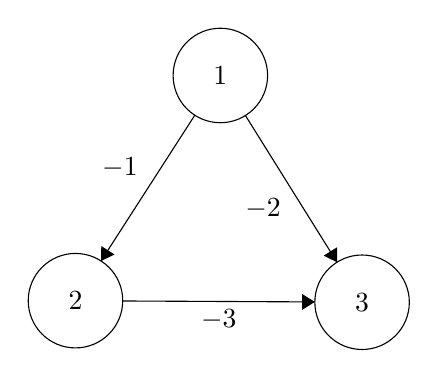
\begin{tikzpicture}[scale=0.2]
\tikzstyle{every node}+=[inner sep=0pt]
\draw [black] (35.9,-16.7) circle (3);
\draw (35.9,-16.7) node {$1$};
\draw [black] (26.7,-31) circle (3);
\draw (26.7,-31) node {$2$};
\draw [black] (44.9,-31.1) circle (3);
\draw (44.9,-31.1) node {$3$};
\draw [black] (34.28,-19.22) -- (28.32,-28.48);
\fill [black] (28.32,-28.48) -- (29.18,-28.07) -- (28.34,-27.53);
\draw (30.68,-22.54) node [left] {$-1$};
\draw [black] (37.49,-19.24) -- (43.31,-28.56);
\fill [black] (43.31,-28.56) -- (43.31,-27.61) -- (42.46,-28.14);
\draw (39.77,-25.19) node [left] {$-2$};
\draw [black] (29.7,-31.02) -- (41.9,-31.08);
\fill [black] (41.9,-31.08) -- (41.1,-30.58) -- (41.1,-31.58);
\draw (35.8,-31.56) node [below] {$-3$};
\end{tikzpicture}
\end{center}


\end{enumerate}

\end{document}
